\chapter{Réalisation du pipeline d'intelligence artificielle et résultats}
\label{chap:realisation-ia}

Ce chapitre rend compte de la réalisation des deux étages d'apprentissage et des
résultats obtenus. Nous décrivons d'abord l'environnement de travail et les jeux de
données, puis la chaîne de préparation. Une section entière est consacrée à la
stratégie d'entraînement, car le dimensionnement du corpus a imposé un arbitrage qui
conditionne la lecture de tous les résultats qui suivent. Nous présentons ensuite les
performances de classification des stades, puis celles de la prédiction de sévérité et
son explicabilité. Le chapitre se clôt sur une discussion des limites
méthodologiques, qui n'est pas un aveu de faiblesse mais une condition de la validité
des conclusions.

% =============================================================================
\section{Environnement de travail}
% =============================================================================

Les entraînements ont été menés sur une station équipée d'un processeur graphique
NVIDIA GeForce RTX 4060 pour portable, disposant de \SI{8,6}{\giga\octet} de mémoire
vidéo, et de \SI{32}{\giga\octet} de mémoire vive. Une seconde station, équipée d'une
RTX 3060, a servi à la construction des ensembles. Le
tableau~\ref{tab:environnement} récapitule l'outillage logiciel.

\begin{table}[H]
\centering
\caption{Environnement logiciel}
\label{tab:environnement}
\small
\begin{tabular}{@{}lL{9.6cm}@{}}
\toprule
\textbf{Domaine} & \textbf{Outils} \\
\midrule
Langage & Python 3.10 \\
Traitement du signal & MNE-Python~\cite{gramfort2013}, SciPy, NumPy \\
Apprentissage profond & PyTorch~\cite{paszke2019} avec accélération CUDA \\
Apprentissage classique & scikit-learn~\cite{pedregosa2011},
XGBoost~\cite{chen2016}, LightGBM~\cite{ke2017} \\
Explicabilité & SHAP~\cite{lundberg2017,lundberg2020} \\
Expérimentation & Jupyter, matplotlib, seaborn \\
\bottomrule
\end{tabular}
\end{table}

% =============================================================================
\section{Jeux de données}
% =============================================================================

\subsection{Sleep-EDF : amorçage du projet}

L'accès aux cohortes cliniques du \emph{National Sleep Research
Resource}~\cite{zhang2018nsrr} est soumis à une autorisation dont l'instruction prend
plusieurs semaines. Plutôt que d'attendre, le premier sprint a été mené sur
\textbf{Sleep-EDF}~\cite{kemp2000}, jeu public diffusé par PhysioNet~\cite{goldberger2000}
et immédiatement téléchargeable.

Ce détour n'a pas produit de résultat rapporté dans ce mémoire : il a servi à valider
la lecture des fichiers, la résolution des dérivations, la segmentation et la boucle
d'entraînement avant même de disposer des données définitives. Lorsque l'autorisation
est arrivée, la chaîne était éprouvée et il n'a plus été question que de la rejouer à
plus grande échelle.

\subsection{SHHS1 : classification des stades}

La \emph{Sleep Heart Health Study}~\cite{quan1997} est une cohorte multicentrique
américaine constituée pour étudier les liens entre troubles respiratoires du sommeil
et risque cardiovasculaire. Sa première visite met à disposition des enregistrements
polysomnographiques complets, accompagnés d'un scorage expert au format XML.

Cent quatre-vingt-seize enregistrements ont été retenus, pour un total de
\num{195130} époques de 30 secondes. Ce nombre n'est pas arbitraire : il résulte de la
contrainte matérielle exposée à la section~\ref{sec:strategie}. Il faut souligner que
le corpus est \textbf{filtré et non échantillonné} : un sujet est écarté s'il lui
manque une des cinq dérivations requises ou son fichier d'annotations. Les sujets
retenus sont donc les premiers de la cohorte à satisfaire le montage complet, ce qui
introduit un biais de sélection dont nous discuterons la portée.

La figure~\ref{fig:distribution} donne la distribution des classes, calculée sur
l'ensemble du corpus.

\begin{figure}[H]
\centering
\begin{tikzpicture}[x=1cm,y=1cm]

  \def\W{11.4}

  % ── Barre 5 classes ───────────────────────────────────────────────────────
  \node[font=\scriptsize\bfseries,text=hypnogray,anchor=east] at (-0.25,1.55)
       {5 classes};
  \foreach \a/\b/\col/\lab/\pct in {
      0/30.70/stWake/W/30{,}7,
      30.70/33.96/stN1/N1/3{,}3,
      33.96/74.13/stN2/N2/40{,}2,
      74.13/87.09/stN3/N3/13{,}0,
      87.09/100/stREM/REM/12{,}9}
  {
    \pgfmathsetmacro{\xa}{\a*\W/100}
    \pgfmathsetmacro{\xb}{\b*\W/100}
    \pgfmathsetmacro{\xm}{(\xa+\xb)/2}
    \fill[\col!75] (\xa,1.15) rectangle (\xb,1.95);
    \draw[white,line width=0.8pt] (\xb,1.15) -- (\xb,1.95);
    \node[font=\tiny\bfseries,text=white] at (\xm,1.68) {\lab};
    \node[font=\tiny,text=white] at (\xm,1.40) {\pct\,\%};
  }

  % ── Barre 3 classes ───────────────────────────────────────────────────────
  \node[font=\scriptsize\bfseries,text=hypnogray,anchor=east] at (-0.25,0.35)
       {3 classes};
  \foreach \a/\b/\col/\lab/\pct in {
      0/30.70/stWake/Wake/30{,}7,
      30.70/87.09/stN2/NREM/56{,}4,
      87.09/100/stREM/REM/12{,}9}
  {
    \pgfmathsetmacro{\xa}{\a*\W/100}
    \pgfmathsetmacro{\xb}{\b*\W/100}
    \pgfmathsetmacro{\xm}{(\xa+\xb)/2}
    \fill[\col!75] (\xa,-0.05) rectangle (\xb,0.75);
    \draw[white,line width=0.8pt] (\xb,-0.05) -- (\xb,0.75);
    \node[font=\tiny\bfseries,text=white] at (\xm,0.48) {\lab};
    \node[font=\tiny,text=white] at (\xm,0.20) {\pct\,\%};
  }

  % ── Annotation ────────────────────────────────────────────────────────────
  \draw[hypnored,line width=0.7pt] (3.50,2.10) -- (3.50,2.45) -- (4.30,2.45);
  \node[font=\scriptsize,text=hypnored,anchor=west] at (4.35,2.45)
       {le N1 ne représente que \num{6361} époques sur \num{195130}};

  \node[font=\tiny\itshape,text=hypnogray,anchor=north] at (5.7,-0.35)
       {corpus SHHS1 --- 196 enregistrements, \num{195130} époques de 30 secondes};

\end{tikzpicture}
\vspace{0.35cm}
\caption[Distribution des stades dans le corpus SHHS1]%
        {Distribution des stades dans le corpus d'entraînement, aux deux granularités.}
\label{fig:distribution}
\end{figure}

Le déséquilibre est frappant et conditionne tout ce qui suit. Le N2 occupe à lui seul
\SI{40,2}{\percent} des époques, tandis que le \textbf{N1 n'en représente que
\SI{3,3}{\percent}}, soit \num{6361} exemples. Un modèle qui ignorerait purement et
simplement cette classe perdrait à peine trois points d'exactitude globale : c'est
exactement le comportement que la pondération des classes vise à empêcher.

\subsection{SHHS2 : prédiction de la sévérité}

La seconde visite de la même cohorte fournit, en plus des hypnogrammes, un index
d'apnées-hypopnées mesuré et un ensemble de variables cliniques. Deux mille six cent
cinquante et un sujets disposent d'un index valide, et \num{2647} d'un hypnogramme
exploitable. La répartition en classes de sévérité, selon les seuils AASM rappelés au
chapitre~\ref{chap:cadre}, est la suivante : \num{629} normaux, \num{960} légers,
\num{637} modérés et \num{425} sévères.

\subsection{MESA}

L'accès à la cohorte \emph{Multi-Ethnic Study of Atherosclerosis} a également été
obtenu, mais elle n'a pas été exploitée faute de temps. Elle constitue le support
naturel d'une validation externe, évoquée en perspective.

% =============================================================================
\section{Chaîne de préparation des données}
% =============================================================================

La préparation est assurée par un script exécuté une seule fois, dont le produit
alimente les douze entraînements. Chaque enregistrement est apparié à son fichier
d'annotations, ses cinq dérivations sont extraites, le signal est ramené à
\SI{100}{\hertz}, découpé en fenêtres de \num{3000} échantillons et centré-réduit
fenêtre par fenêtre. Le résultat est sérialisé sous forme d'un tenseur en simple
précision accompagné d'un vecteur d'étiquettes en entier court, soit environ
\SI{60}{\mega\octet} par nuit.

Quatre décisions de traitement méritent d'être explicitées.

\paragraph{Sélection stricte des dérivations.} À l'entraînement, les cinq dérivations
sont exigées sous leur dénomination exacte et tout écart écarte le sujet. En
production, au contraire, une table d'alias couvre les conventions de nommage des
différents constructeurs et replie sur l'EEG principal une dérivation absente. Cette
asymétrie est voulue : sélectivité pour la pureté du corpus d'apprentissage,
tolérance pour l'interopérabilité clinique.

\paragraph{Fusion des anciens stades 3 et 4.} Les annotations de SHHS suivent encore
la nomenclature de Rechtschaffen et Kales~\cite{rechtschaffen1968}. Le stade 4 est
fusionné dans le N3, conformément à la révision AASM de 2007.

\paragraph{Comblement des époques non scorées.} Les fenêtres sans stade attribué
reçoivent le dernier stade valide observé ; celles qui précèdent le premier stade
scoré sont considérées comme de l'éveil. Cette dernière convention est une hypothèse —
l'enregistrement débute avant l'extinction des lumières — et non une donnée.

\paragraph{Normalisation locale.} Comme exposé au chapitre~\ref{chap:conception}, la
statistique de centrage et de réduction est calculée sur chaque fenêtre isolément.
Aucune statistique globale n'étant estimée sur le corpus, la normalisation ne peut
véhiculer aucune information de l'ensemble d'entraînement vers l'ensemble de test.

Le corpus est ensuite découpé en trois parts stratifiées sur la classe, dans les
proportions \num{80} / \num{10} / \num{10}, soit \num{156104} époques d'entraînement
et \num{19513} pour chacun des ensembles de validation et de test. La pondération des
classes est fixée à l'inverse de leur fréquence, puis renormalisée : le REM se voit
attribuer un poids \num{4,4} fois supérieur à celui du NREM en trois classes, et le N1
un poids \num{12,3} fois supérieur à celui du N2 en cinq classes.

% =============================================================================
\section{Stratégie d'entraînement et contraintes matérielles}
\label{sec:strategie}
% =============================================================================

\subsection{Dimensionnement du problème}

Une époque de 30 secondes échantillonnée à \SI{100}{\hertz} sur cinq dérivations
occupe \SI{60}{\kilo\octet} en simple précision. Rapporté à une cohorte entière, le
corpus dépasse de plusieurs ordres de grandeur ce qu'une station de développement peut
contenir. Le tableau~\ref{tab:empreinte} donne les chiffres.

\begin{table}[H]
\centering
\caption{Empreinte du corpus d'entraînement en simple précision}
\label{tab:empreinte}
\small
\begin{tabular}{@{}L{5.0cm}rrrl@{}}
\toprule
\textbf{Configuration} & \textbf{Sujets} & \textbf{Époques} & \textbf{Empreinte} &
\textbf{Tient dans} \\
\midrule
2 dérivations & 196 & \num{195130} & \SI{4,7}{\giga\octet} & mémoire vidéo et vive \\
5 dérivations & 196 & \num{195130} & \SI{11,7}{\giga\octet} & mémoire vive seulement \\
5 dérivations, variante attentionnelle & 150 & \num{148958} & \SI{8,9}{\giga\octet} &
mémoire vive seulement \\
\textbf{cohorte SHHS1 complète} & \num{5793} & $\approx$ \num{5800000} &
$\approx$ \SI{346}{\giga\octet} & ni l'une ni l'autre \\
\bottomrule
\end{tabular}
\end{table}

La cohorte complète représenterait environ \SI{346}{\giga\octet}. Comme les fichiers
préparés sont stockés exactement tels qu'ils seront chargés, ce chiffre vaut aussi bien
pour le disque que pour la mémoire : la contrainte se manifeste deux fois, dès la
préparation. La question n'est donc pas « toutes les données ou pas », mais
\emph{quelle fraction} convertir et \emph{comment} la faire circuler jusqu'au
processeur graphique.

\subsection{Trois stratégies de résidence des données}

Trois options ont été évaluées, résumées au tableau~\ref{tab:residence}.

\begin{table}[H]
\centering
\caption{Stratégies de résidence des données pendant l'entraînement}
\label{tab:residence}
\small
\begin{tabular}{@{}L{2.9cm}L{4.5cm}L{4.3cm}c@{}}
\toprule
\textbf{Stratégie} & \textbf{Principe} & \textbf{Limite} & \textbf{Décision} \\
\midrule
Tout en mémoire vidéo &
Le corpus est transféré une fois sur le processeur graphique ; plus aucune copie
pendant l'entraînement &
Ne laisse pas de marge pour les activations et exclut d'emblée le protocole à cinq
dérivations & écartée \\
\addlinespace[3pt]
\textbf{Tout en mémoire vive} &
Le corpus réside dans la mémoire de l'hôte ; chaque lot est copié vers le processeur
graphique en accès direct depuis une zone page-verrouillée &
Plafonne le nombre de sujets ; empreinte doublée au moment du découpage &
\textbf{retenue} \\
\addlinespace[3pt]
Lecture paresseuse &
Chaque lot est relu sur disque à la volée ; l'empreinte mémoire devient négligeable &
Le processeur graphique attend le disque à chaque itération &
écartée \\
\bottomrule
\end{tabular}
\end{table}

\subsection{L'arbitrage retenu}

La lecture paresseuse aurait permis d'exploiter les \num{5793} enregistrements, mais
en affamant le processeur graphique : le temps par époque devient dominé par les
entrées-sorties. Dans les quatre semaines du sprint de modélisation, il aurait fallu
descendre bien en dessous des trente époques d'entraînement nécessaires à la
convergence, et cela pour douze variantes. Le modèle aurait vu davantage de patients,
mais chacun beaucoup moins souvent, et aurait sous-appris.

Le choix inverse a été fait : \textbf{restreindre la cohorte à 196 sujets pour que le
corpus tienne intégralement en mémoire vive}, et consacrer la totalité du budget de
calcul à l'apprentissage plutôt qu'au transfert. Les \num{195130} exemples étiquetés
restent largement suffisants pour des architectures de quelques millions de
paramètres, et les trente époques complètes ont pu être menées sur les douze variantes.

\subsection{La contrainte était réelle : le cas du modèle attentionnel}

Onze carnets sur douze fixent la limite à 196 sujets. Le douzième — le modèle
attentionnel à cinq dérivations et trois classes — descend à \textbf{150}, soit
\num{148958} époques et \SI{8,9}{\giga\octet}. Ce modèle matérialise soixante jetons de
dimension 128 par époque, ainsi qu'une matrice d'attention par tête : ses activations
débordaient là où les deux autres architectures passaient encore.

Cette réduction explique un écart qu'il faut signaler pour qu'il ne passe pas pour une
erreur : le jeu de test de cette seule variante compte \num{14896} époques au lieu de
\num{19513}.

\subsection{Optimisations et boucle d'entraînement}

Le tableau~\ref{tab:optim} récapitule les réglages retenus et leur raison d'être.

\begin{table}[H]
\centering
\caption{Réglages d'entraînement}
\label{tab:optim}
\small
\begin{tabular}{@{}L{4.0cm}L{10.0cm}@{}}
\toprule
\textbf{Réglage} & \textbf{Effet recherché} \\
\midrule
Précision mixte & Activations en demi-précision, accumulations en simple précision,
avec mise à l'échelle des gradients : environ deux fois moins de mémoire
d'activations et un gain de débit sur les unités tensorielles \\
\addlinespace[2pt]
Mémoire page-verrouillée & Copie en accès direct vers le processeur graphique,
recouvrant le calcul du lot précédent \\
\addlinespace[2pt]
Aucun processus de chargement parallèle & Choix contre-intuitif mais adapté : les
données étant déjà en mémoire, un processus supplémentaire dupliquerait le tenseur de
\SI{11,7}{\giga\octet} sans rien précharger \\
\addlinespace[2pt]
Segments extensibles & Limite la fragmentation de l'allocateur, source d'échecs
d'allocation en fin d'entraînement \\
\addlinespace[2pt]
Optimiseur AdamW, pas initial \num{5e-4} & Découplage de la régularisation et de
l'adaptation du pas \\
\addlinespace[2pt]
Recuit cosinus sur 30 époques & Décroissance progressive du pas jusqu'à \num{1e-6} \\
\addlinespace[2pt]
Écrêtage du gradient à \num{1,0} & Indispensable au modèle récurrent, où les gradients
explosent sur des séquences de \num{3000} pas \\
\addlinespace[2pt]
Sélection sur le $\kappa$ de validation & Sur des classes déséquilibrées, la perte peut
s'améliorer pendant que la classe minoritaire se dégrade ; le $\kappa$ de
Cohen~\cite{cohen1960} ne le permet pas \\
\bottomrule
\end{tabular}
\end{table}

La figure~\ref{fig:courbes} illustre le déroulement d'un entraînement.

\begin{figure}[H]
\centering
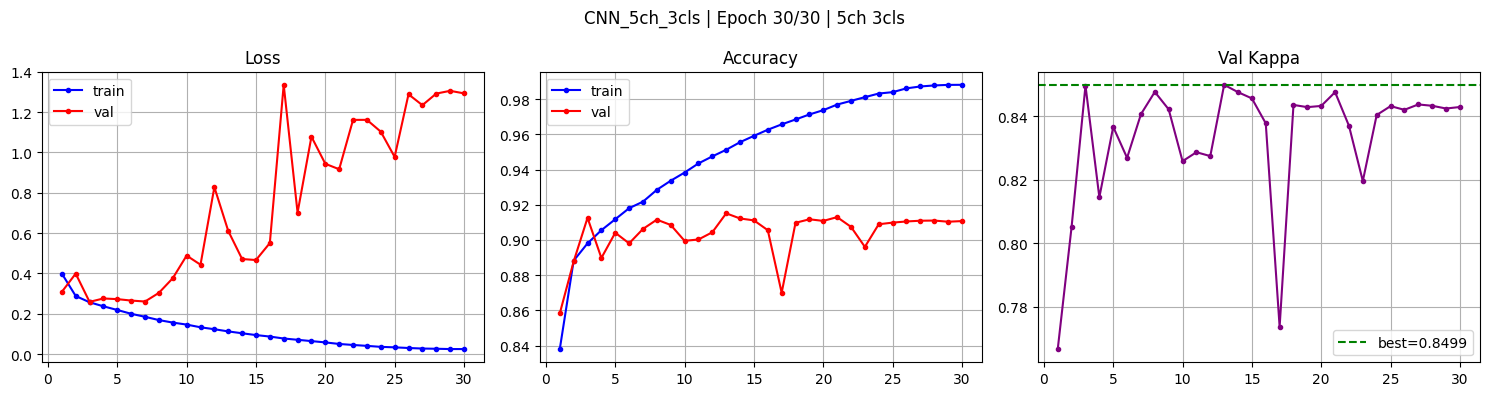
\includegraphics[width=\textwidth]{images/resultats/curves_CNN_5ch_3cls.png}
\caption[Courbes d'apprentissage du modèle convolutif]%
        {Évolution de la perte, de l'exactitude et du $\kappa$ de validation au cours
         des trente époques d'entraînement du modèle convolutif à cinq dérivations et
         trois classes.}
\label{fig:courbes}
\end{figure}

L'écart croissant entre les courbes d'entraînement et de validation traduit un
surapprentissage progressif, que la sélection du meilleur point de contrôle sur le
$\kappa$ de validation neutralise en pratique.

% =============================================================================
\section{Résultats de la classification des stades}
% =============================================================================

\subsection{Les douze modèles de base}

Chaque architecture a été entraînée sur les quatre combinaisons de montage et de
granularité, soit douze modèles au total. Le tableau~\ref{tab:12modeles} présente les
résultats sur le jeu de test.

\begin{table}[H]
\centering
\caption{Performances des douze modèles de base sur le jeu de test}
\label{tab:12modeles}
\small
\begin{tabular}{@{}llcccc@{}}
\toprule
\textbf{Configuration} & \textbf{Architecture} & \textbf{Exactitude} &
\textbf{$\kappa$} & \textbf{F1 macro} & \textbf{F1 pondéré} \\
\midrule
\multirow{3}{*}{5 dérivations, 3 classes}
 & Convolutif   & \textbf{\SI{91,66}{\percent}} & \textbf{0,853} & 0,89 & 0,92 \\
 & Récurrent    & \SI{90,86}{\percent} & 0,843 & 0,89 & 0,91 \\
 & Attentionnel & \SI{90,14}{\percent} & 0,826 & 0,87 & 0,90 \\
\midrule
\multirow{3}{*}{2 dérivations, 3 classes}
 & Convolutif   & \SI{89,10}{\percent} & 0,810 & 0,86 & 0,89 \\
 & Récurrent    & \SI{87,58}{\percent} & 0,790 & 0,84 & 0,88 \\
 & Attentionnel & \SI{86,92}{\percent} & 0,771 & 0,83 & 0,87 \\
\midrule
\multirow{3}{*}{5 dérivations, 5 classes}
 & Convolutif   & \SI{82,78}{\percent} & 0,761 & 0,72 & 0,83 \\
 & Récurrent    & \SI{78,60}{\percent} & 0,713 & 0,71 & 0,80 \\
 & Attentionnel & \SI{81,55}{\percent} & 0,742 & 0,70 & 0,81 \\
\midrule
\multirow{3}{*}{2 dérivations, 5 classes}
 & Convolutif   & \SI{79,90}{\percent} & 0,723 & 0,69 & 0,80 \\
 & Récurrent    & \SI{76,01}{\percent} & 0,679 & 0,68 & 0,78 \\
 & Attentionnel & \SI{77,15}{\percent} & 0,686 & 0,66 & 0,77 \\
\bottomrule
\end{tabular}
\end{table}

Trois enseignements se dégagent.

\paragraph{L'apport des dérivations oculaires et musculaires est net.} À granularité
constante, le passage de deux à cinq dérivations gagne entre \num{2,6} et
\num{3,9} points d'exactitude. Ce résultat était attendu : l'électro-oculogramme et
l'électromyogramme portent précisément l'information qui distingue le sommeil
paradoxal, et le référentiel AASM les exige pour cette raison.

\paragraph{Le passage à cinq stades coûte cher.} La même architecture perd entre
\num{8,6} et \num{12,3} points en passant de trois à cinq classes. Le
tableau~\ref{tab:parclasse} montre où se situe la perte.

\paragraph{Le convolutif domine, mais de peu.} Il arrive en tête sur les quatre
configurations. L'écart avec les deux autres architectures reste toutefois inférieur à
quatre points, ce qui confirme l'observation faite au chapitre~\ref{chap:etat-art} :
aucune famille ne domine franchement, et leurs erreurs ne sont pas identiques.

La figure~\ref{fig:cm-3archi} rend cette dernière affirmation visible. Les trois
matrices portent sur le même jeu de test, mais leurs erreurs ne se situent pas aux
mêmes endroits : le modèle récurrent confond davantage le NREM avec le REM, tandis
que le convolutif se trompe plutôt sur l'éveil. C'est cette complémentarité que
l'empilement exploite.

\begin{figure}[H]
\centering
\begin{subfigure}[t]{0.325\textwidth}
  \centering
  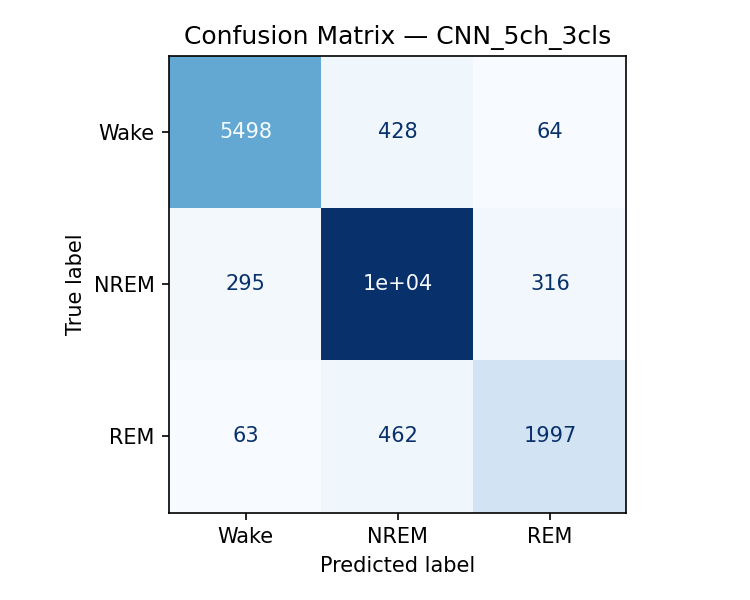
\includegraphics[width=\linewidth]{images/resultats/cm_CNN_5ch_3cls.png}
  \caption{Convolutif}
\end{subfigure}
\hfill
\begin{subfigure}[t]{0.325\textwidth}
  \centering
  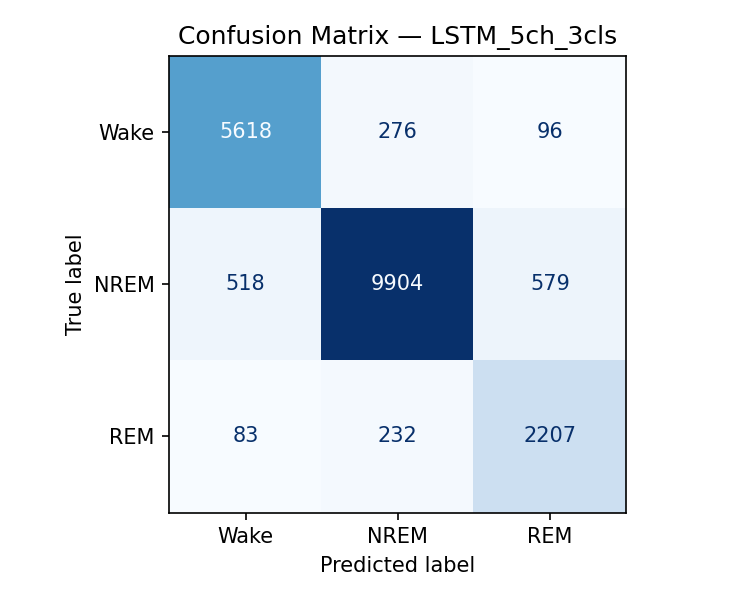
\includegraphics[width=\linewidth]{images/resultats/cm_LSTM_5ch_3cls.png}
  \caption{Récurrent}
\end{subfigure}
\hfill
\begin{subfigure}[t]{0.325\textwidth}
  \centering
  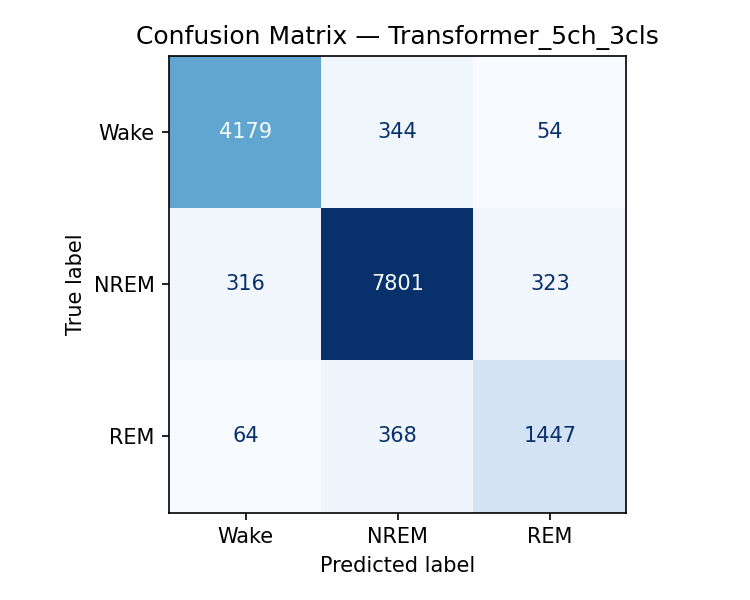
\includegraphics[width=\linewidth]{images/resultats/cm_Transformer_5ch_3cls.png}
  \caption{Attentionnel}
\end{subfigure}
\caption[Matrices de confusion des trois architectures]%
        {Matrices de confusion des trois architectures, configuration à cinq
         dérivations et trois classes. Effectifs bruts.}
\label{fig:cm-3archi}
\end{figure}

\subsection{Le problème du stade N1}

\begin{table}[H]
\centering
\caption{Performances par classe --- configuration à cinq dérivations}
\label{tab:parclasse}
\small
\begin{tabular}{@{}llcccc@{}}
\toprule
& \textbf{Classe} & \textbf{Précision} & \textbf{Rappel} & \textbf{F1} &
\textbf{Effectif} \\
\midrule
\multirow{3}{*}{\rotatebox{90}{\scriptsize 3 classes}}
 & Éveil & 0,94 & 0,92 & 0,93 & \num{5990} \\
 & NREM  & 0,92 & 0,94 & 0,93 & \num{11001} \\
 & REM   & 0,84 & 0,79 & 0,82 & \num{2522} \\
\midrule
\multirow{5}{*}{\rotatebox{90}{\scriptsize 5 classes}}
 & Éveil & 0,92 & 0,92 & 0,92 & \num{5990} \\
 & N1    & \textcolor{hypnored}{\textbf{0,29}} &
           \textcolor{hypnored}{\textbf{0,24}} &
           \textcolor{hypnored}{\textbf{0,26}} & \num{638} \\
 & N2    & 0,86 & 0,78 & 0,82 & \num{7832} \\
 & N3    & 0,70 & 0,88 & 0,78 & \num{2531} \\
 & REM   & 0,80 & 0,84 & 0,82 & \num{2522} \\
\bottomrule
\end{tabular}
\end{table}

Le constat est sans appel : \textbf{le stade N1 est la seule classe véritablement
échouée}, avec un F1 de \num{0,26} pour le modèle convolutif. Les autres architectures
ne font pas mieux — le récurrent atteint \num{0,30} et l'attentionnel \num{0,21} —
mais elles échouent différemment. Le récurrent affiche un rappel de \num{0,59} pour une
précision de \num{0,20} : il sur-prédit massivement le N1. Le convolutif fait
l'inverse, avec un rappel de \num{0,24} pour une précision de \num{0,29}.

La figure~\ref{fig:cm-5cls} montre où partent les époques de N1 mal classées.

\begin{figure}[H]
\centering
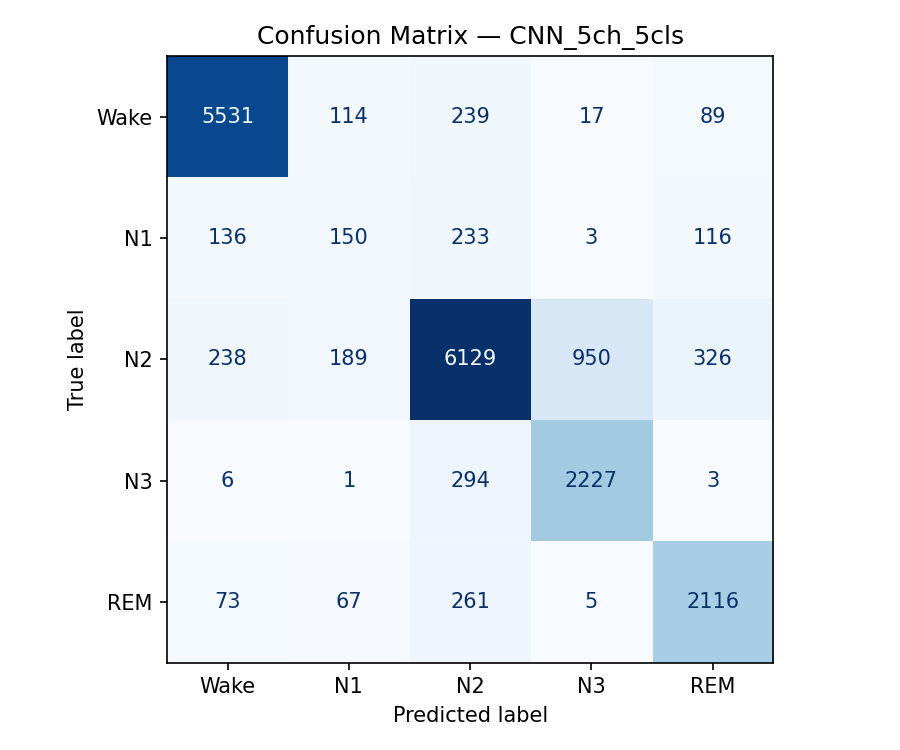
\includegraphics[width=0.72\textwidth]{images/resultats/cm_CNN_5ch_5cls.png}
\caption[Matrice de confusion à cinq classes]%
        {Matrice de confusion du modèle convolutif à cinq dérivations et cinq
         classes. Effectifs bruts sur les \num{19513} époques de test.}
\label{fig:cm-5cls}
\end{figure}

Sur les \num{638} époques réellement en N1, \num{150} seulement sont reconnues. Les
autres se dispersent : \num{233} sont versées en N2, \num{136} en éveil et \num{116}
en sommeil paradoxal. Cette dispersion n'est pas un défaut d'apprentissage mais le
reflet de la définition même du stade — un état de transition entre l'éveil et le
sommeil installé, sans marqueur graphique propre. Le modèle le classe dans les états
qui l'encadrent, ce que fait aussi un scoreur humain hésitant.

On observe par ailleurs une seconde confusion, de nature différente : \num{950} époques
de N2 sont classées en N3. Celle-ci relève d'un seuil et non d'une ambiguïté — le
référentiel AASM fixe le passage en N3 à \SI{20}{\percent} d'ondes lentes dans la
fenêtre, et une époque à \SI{19}{\percent} est presque indiscernable d'une époque à
\SI{21}{\percent}.

Cette divergence est instructive. Elle confirme d'abord que les erreurs des deux
familles ne se recouvrent pas, ce qui est la condition d'efficacité de l'empilement.
Elle rejoint ensuite ce que la littérature établit et que nous avons rappelé au
chapitre~\ref{chap:cadre} : le N1 est un état de transition défini négativement, sur
lequel les experts humains eux-mêmes s'accordent le moins~\cite{rosenberg2013}. Avec
\num{638} exemples de test pour \num{6361} exemples d'entraînement, la rareté aggrave
la difficulté intrinsèque.

\subsection{Les quatre ensembles}

Le tableau~\ref{tab:ensembles} présente les résultats des ensembles, comparés à leurs
modèles constitutifs et au vote moyen.

\begin{table}[H]
\centering
\caption{Ensembles par empilement, comparés aux modèles de base et au vote moyen}
\label{tab:ensembles}
\small
\begin{tabular}{@{}lcccccc@{}}
\toprule
\textbf{Configuration} & \textbf{Conv.} & \textbf{Réc.} & \textbf{Att.} &
\textbf{Vote moyen} & \textbf{Empilement} & \textbf{Gain} \\
\midrule
5 dérivations, 3 classes & 0,932 & 0,875 & 0,944 & \textbf{0,950} & 0,947 &
\textcolor{hypnored}{$-$0,003} \\
2 dérivations, 3 classes & 0,863 & 0,821 & 0,918 & 0,917 & \textbf{0,924} & $+$0,006 \\
5 dérivations, 5 classes & 0,875 & 0,754 & 0,887 & 0,894 & \textbf{0,899} & $+$0,005 \\
2 dérivations, 5 classes & 0,819 & 0,695 & 0,815 & 0,834 & \textbf{0,839} & $+$0,005 \\
\bottomrule
\end{tabular}
\vspace{2pt}
\raggedright\footnotesize
Valeurs de $\kappa$ de Cohen sur le jeu de test par sujets. Le gain est mesuré par
rapport au vote moyen.
\end{table}

Ces résultats appellent une lecture nuancée, et c'est précisément ce qui les rend
intéressants.

L'empilement \textbf{dépasse le meilleur modèle isolé sur les quatre configurations},
ce qui valide le principe. Mais il \textbf{ne dépasse le vote moyen que sur trois
configurations sur quatre} : sur la variante à cinq dérivations et trois classes,
la moyenne arithmétique des probabilités fait légèrement mieux que le méta-apprenant.

L'explication tient à la taille du jeu d'apprentissage du second niveau. Le
méta-apprenant est entraîné sur les probabilités produites sur l'ensemble de
validation, soit une vingtaine de milliers d'exemples décrits par neuf variables
seulement. Lorsque les trois modèles de base sont déjà très concordants — ce qui est le
cas dans la configuration la plus favorable — il ne reste presque rien à apprendre, et
la pondération estimée n'apporte pas davantage qu'une moyenne uniforme.

Un mémoire qui n'aurait rapporté que le gain sur le meilleur modèle isolé aurait
présenté l'empilement comme systématiquement supérieur. La comparaison au vote moyen,
souvent omise dans la littérature, montre que son apport est réel mais modeste, et
qu'il dépend du degré de désaccord entre les modèles combinés.

\begin{figure}[H]
\centering
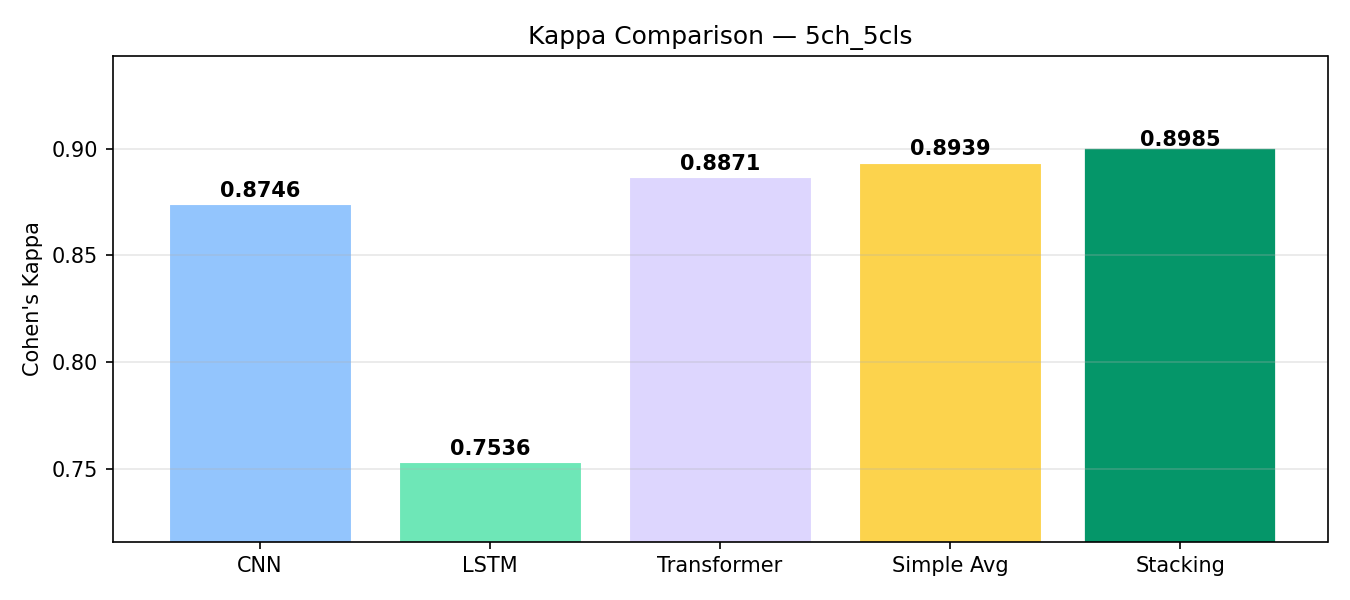
\includegraphics[width=0.92\textwidth]{images/resultats/kappa_comparison_5ch_5cls.png}
\caption[Comparaison des $\kappa$ pour l'ensemble à cinq classes]%
        {Comparaison des $\kappa$ obtenus par les modèles de base, le vote moyen et
         l'empilement, pour la configuration à cinq dérivations et cinq classes.}
\label{fig:kappa-comp}
\end{figure}

La figure~\ref{fig:cm-stack} présente la matrice de confusion de l'ensemble le plus
performant.

\begin{figure}[H]
\centering
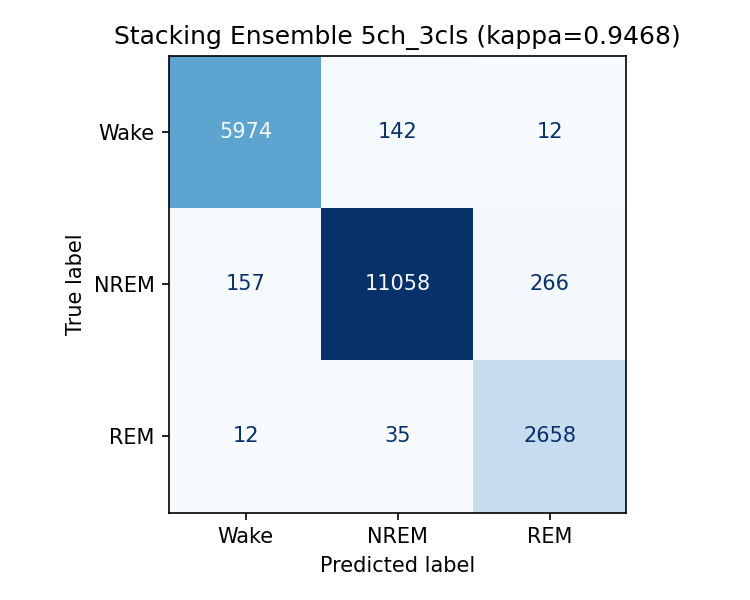
\includegraphics[width=0.62\textwidth]{images/resultats/cm_stacking_5ch_3cls.png}
\caption[Matrice de confusion de l'ensemble]%
        {Matrice de confusion de l'ensemble à cinq dérivations et trois classes, sur
         les \num{20314} époques du jeu de test par sujets.}
\label{fig:cm-stack}
\end{figure}

Les comparaisons pour les trois autres configurations, ainsi que les matrices de
confusion correspondantes, figurent en annexe~\ref{annexe:staging}.

% =============================================================================
\section{Résultats de la prédiction de sévérité}
% =============================================================================

\subsection{Protocole}

Les marqueurs d'architecture ont été extraits de \num{2647} hypnogrammes, puis
complétés des variables cliniques et des variables d'interaction, pour un total de
\textbf{53 variables}. Le jeu a été partagé en \SI{80}{\percent} d'apprentissage et
\SI{20}{\percent} de test, soit \num{530} sujets de test, avec stratification sur la
classe de sévérité.

Deux précautions méthodologiques ont été prises. Les \textbf{index de perturbation
respiratoire ont été exclus} des variables d'entrée : ils mesurent directement les
événements dont on cherche à prédire la sévérité, et les conserver aurait produit un
modèle excellent mais dépourvu de valeur pratique. Par ailleurs, les modèles sensibles
à l'échelle — machine à vecteurs de support, plus proches voisins, perceptron
multicouche — ont été encapsulés avec leur normaliseur dans un pipeline, de sorte que
celui-ci soit ajusté sur chaque pli d'entraînement seulement et jamais sur le pli
d'évaluation.

La figure~\ref{fig:distrib-osa} montre comment quelques marqueurs d'architecture se
comportent selon la classe de sévérité. On y lit à la fois la validité de l'hypothèse
de départ — l'efficacité du sommeil décroît et l'index de fragmentation croît avec la
sévérité — et la difficulté de la tâche : les distributions des classes normale et
légère se recouvrent presque entièrement.

\begin{figure}[H]
\centering
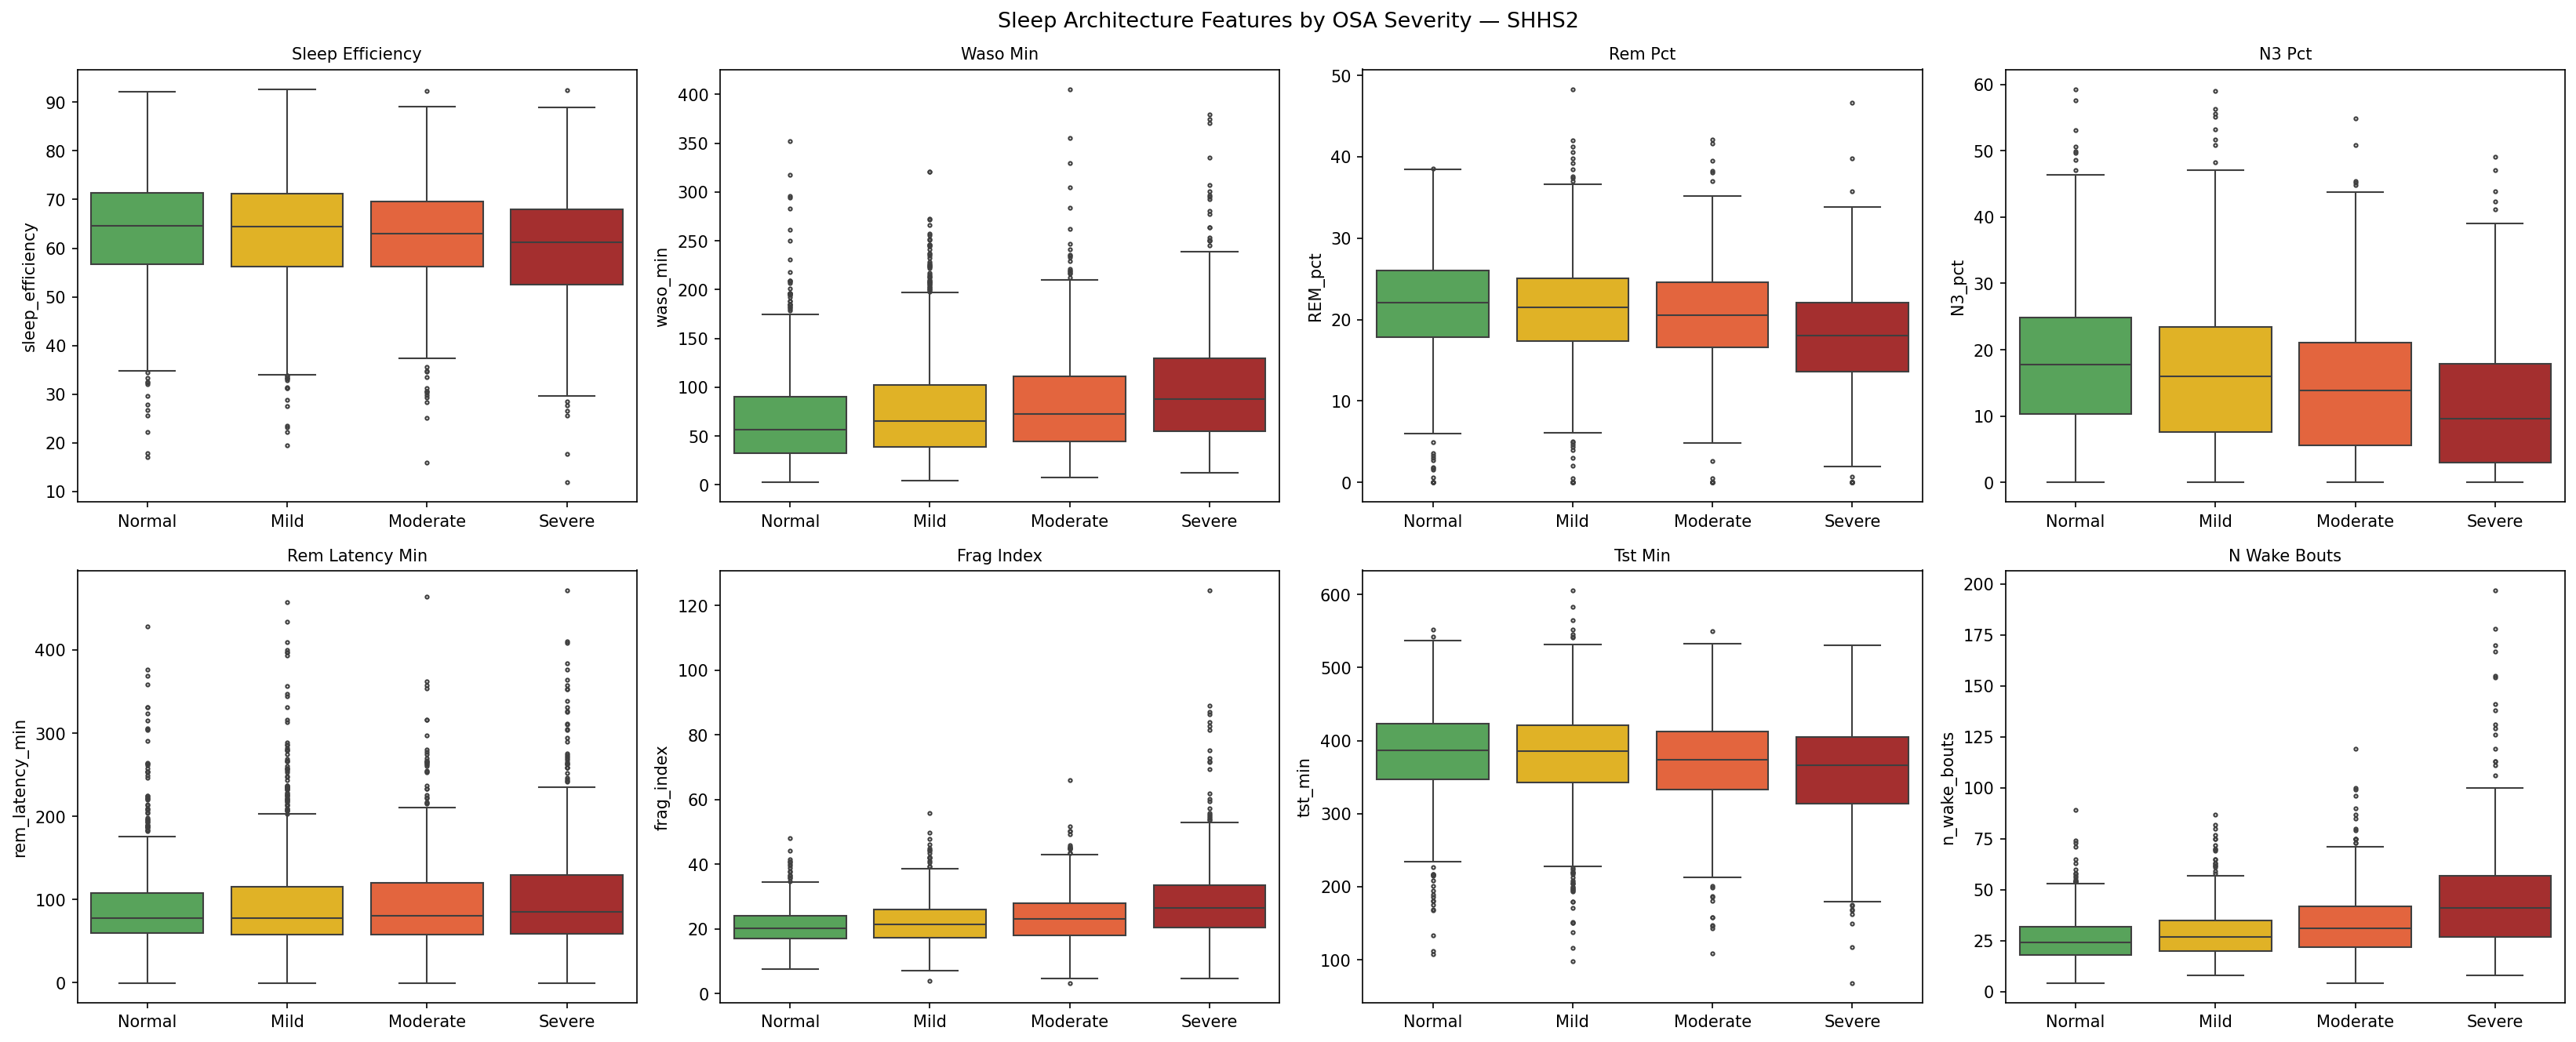
\includegraphics[width=\textwidth]{images/resultats/feature_distributions.png}
\caption[Distribution des marqueurs selon la sévérité]%
        {Distribution de huit marqueurs d'architecture du sommeil selon la classe de
         sévérité, sur la cohorte SHHS2.}
\label{fig:distrib-osa}
\end{figure}

\subsection{Comparaison des six classifieurs}

Six familles ont été comparées en validation croisée stratifiée à cinq plis, sur le
F1 macro (figure~\ref{fig:comparaison-osa}).

\begin{figure}[H]
\centering
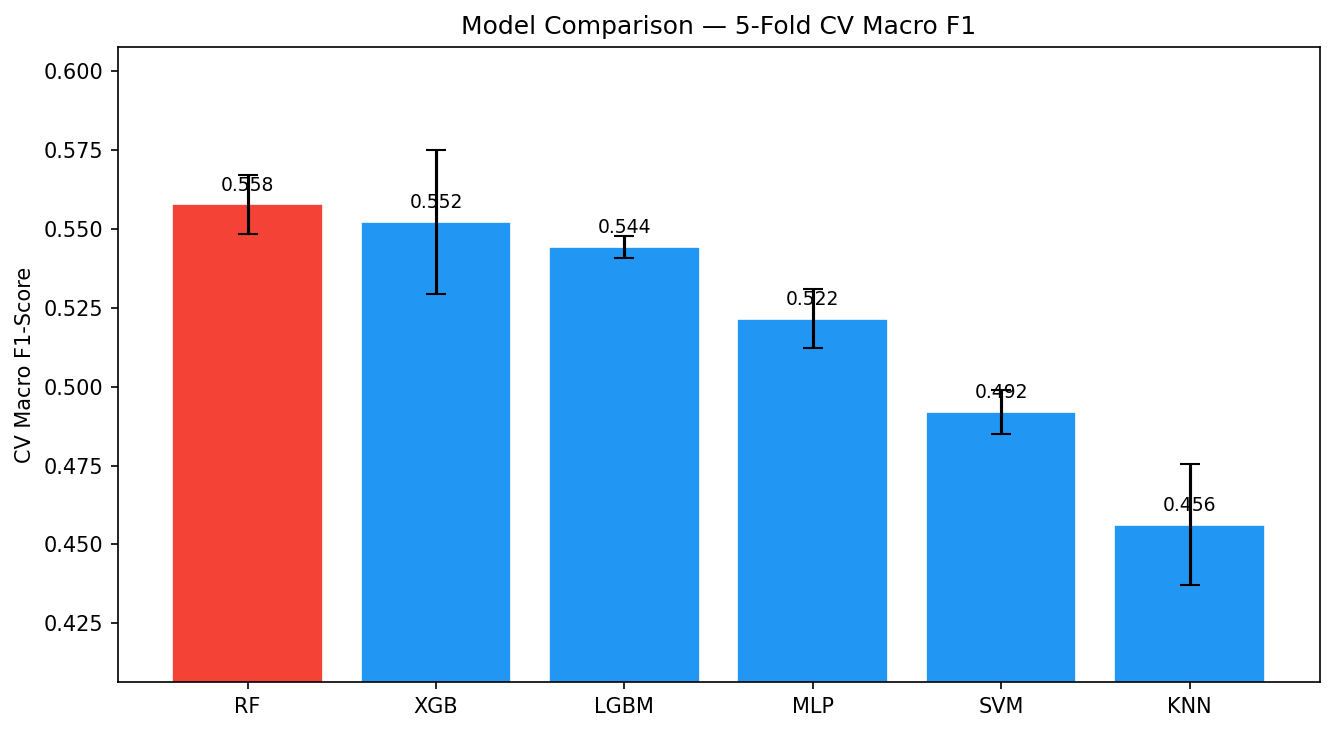
\includegraphics[width=0.88\textwidth]{images/resultats/model_comparison.png}
\caption[Comparaison des six classifieurs en validation croisée]%
        {F1 macro en validation croisée à cinq plis. La forêt aléatoire arrive en
         tête, suivie des deux implémentations de gradient boosté.}
\label{fig:comparaison-osa}
\end{figure}

La forêt aléatoire obtient le meilleur score (\num{0,558}), suivie de près par
XGBoost (\num{0,552}) et LightGBM (\num{0,544}). Le perceptron multicouche
(\num{0,522}), la machine à vecteurs de support (\num{0,492}) et les plus proches
voisins (\num{0,456}) suivent. Les trois premiers ont été retenus comme modèles de
base de l'ensemble, dont le méta-apprenant est une régression logistique équilibrée.

\subsection{Performances sur le jeu de test}

Le tableau~\ref{tab:osa-resultats} confronte la meilleure ligne de base et l'ensemble.

\begin{table}[H]
\centering
\caption{Prédiction de la sévérité --- résultats sur les 530 sujets de test}
\label{tab:osa-resultats}
\small
\begin{tabular}{@{}lcccc@{}}
\toprule
\textbf{Modèle} & \textbf{Exactitude} & \textbf{$\kappa$} & \textbf{F1 macro} &
\textbf{Écart $\leq$ 1 classe} \\
\midrule
Forêt aléatoire & \textbf{\SI{57,0}{\percent}} & \textbf{0,409} & \textbf{0,576} &
\SI{95,5}{\percent} \\
Empilement & \SI{54,5}{\percent} & 0,389 & 0,558 & \SI{95,3}{\percent} \\
\midrule
\emph{Référence : classe majoritaire} & \SI{36,2}{\percent} & 0,000 & 0,133 & --- \\
\bottomrule
\end{tabular}
\end{table}

Ces résultats méritent d'être commentés sans complaisance.

\paragraph{L'empilement n'apporte rien ici.} Contrairement au cas de la
classification des stades, il fait légèrement \emph{moins} bien que la meilleure
ligne de base. Ce résultat négatif est cohérent avec la condition de diversité posée au
chapitre~\ref{chap:etat-art} : les trois modèles retenus sont tous des ensembles
d'arbres, entraînés sur les mêmes variables. Leurs erreurs se recouvrent largement, et
la combinaison n'a rien à corriger. Retenir la forêt aléatoire seule serait ici le
choix rationnel.

\paragraph{La tâche est intrinsèquement difficile.} Une exactitude de
\SI{57}{\percent} sur quatre classes peut sembler faible, mais la référence par la
classe majoritaire n'est que de \SI{36,2}{\percent}, et le $\kappa$ de \num{0,41}
correspond à un accord modéré. La difficulté vient de la nature même des seuils :
un index d'apnées de \num{4,9} et un index de \num{5,1} classent deux patients
différemment alors que rien ne les distingue physiologiquement. La frontière entre
normal et léger est conventionnelle, non biologique.

\paragraph{L'erreur est presque toujours de faible amplitude.} Plus de
\SI{95}{\percent} des prédictions tombent dans la bonne classe ou dans une classe
adjacente. C'est la statistique cliniquement pertinente : le système se trompe
rarement de plus d'un cran de sévérité, et n'annonce quasiment jamais un patient
sévère comme normal.

Les courbes ROC en un-contre-tous (figure~\ref{fig:roc-osa}) confirment cette lecture :
les classes extrêmes — normale et sévère — sont nettement mieux séparées que les deux
classes intermédiaires.

\begin{figure}[H]
\centering
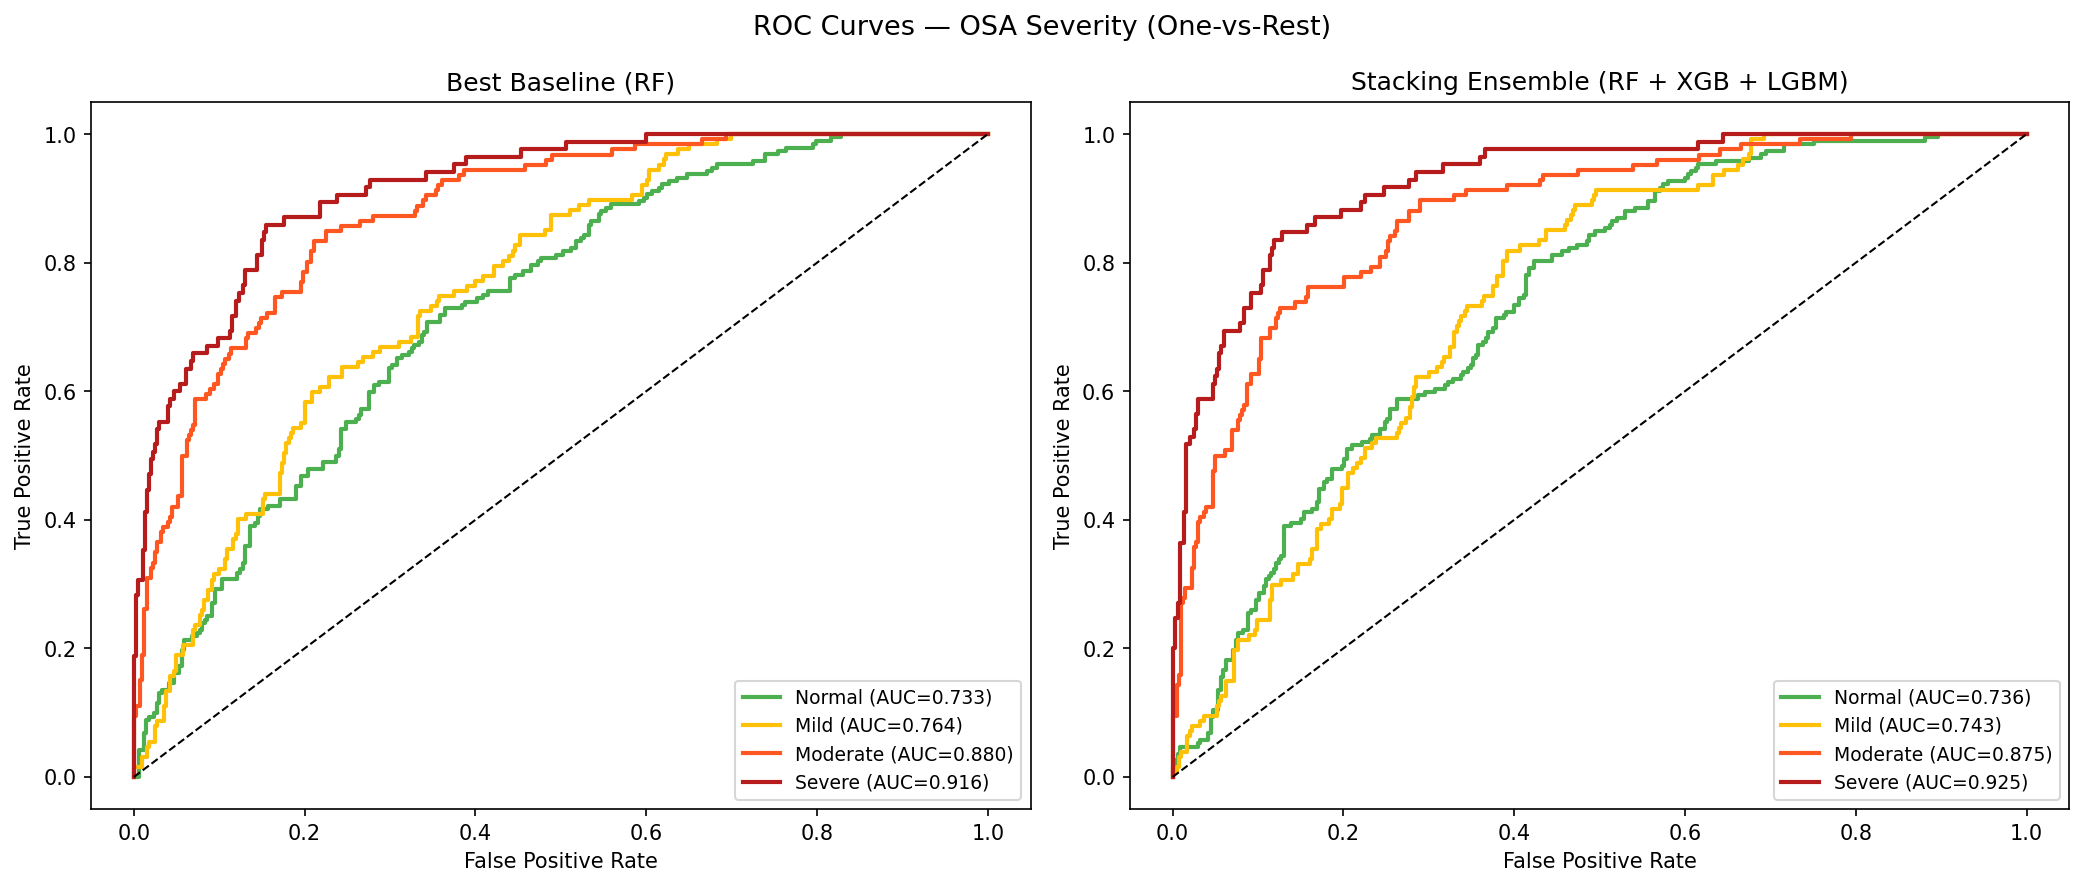
\includegraphics[width=\textwidth]{images/resultats/roc_curves.png}
\caption[Courbes ROC de la prédiction de sévérité]%
        {Courbes ROC en un-contre-tous, meilleure ligne de base et ensemble.}
\label{fig:roc-osa}
\end{figure}

\begin{samepage}
\noindent\textbf{Avertissement sur les étiquettes.} Les figures produites par le script
d'origine portaient des étiquettes d'axes erronées : l'encodeur de classes de
scikit-learn les trie par ordre alphabétique, si bien que l'ordre effectif des indices
est \emph{Léger, Modéré, Normal, Sévère} et non l'ordre de sévérité utilisé dans le
code. Le défaut ne touchait que l'affichage — les prédictions du système sont
correctes — mais il a été corrigé dans le script, et les matrices de confusion
présentées dans ce mémoire ont été recalculées avec l'ordre exact.
\end{samepage}

La figure~\ref{fig:cm-osa} détaille la structure des confusions.

\begin{figure}[H]
\centering
\begin{tikzpicture}[x=1.28cm,y=1.02cm,font=\scriptsize]

  \def\CM{
    {83,38,3,2},
    {39,109,35,9},
    {4,47,54,22},
    {0,6,23,56}}

  \foreach \lab [count=\j from 0] in {Normal,Léger,Modéré,Sévère}
    \node[font=\scriptsize,anchor=base] at (\j+0.5,4.14) {\lab};
  \foreach \lab [count=\i from 0] in {Normal,Léger,Modéré,Sévère}
    \node[font=\scriptsize,anchor=east] at (-0.08,3.5-\i) {\lab};

  \foreach \row [count=\i from 0] in \CM {
    \foreach \v [count=\j from 0] in \row {
      \pgfmathsetmacro{\tot}{\i==0 ? 126 : (\i==1 ? 192 : (\i==2 ? 127 : 85))}
      \pgfmathsetmacro{\int}{100*\v/\tot}
      \pgfmathsetmacro{\diag}{\i==\j ? 1 : 0}
      \ifnum\diag=1
        \fill[hypnoblue!\int] (\j,3-\i) rectangle (\j+1,4-\i);
      \else
        \fill[hypnored!\int] (\j,3-\i) rectangle (\j+1,4-\i);
      \fi
      \draw[white,line width=0.9pt] (\j,3-\i) rectangle (\j+1,4-\i);
      \node[font=\scriptsize] at (\j+0.5,3.5-\i) {\v};
    }
  }

  \node[font=\scriptsize\itshape,anchor=north] at (2.0,-0.25) {classe prédite};
  \node[font=\scriptsize\itshape,rotate=90] at (-1.35,2.0) {classe réelle};

\end{tikzpicture}
\vspace{0.3cm}
\caption[Matrice de confusion de la prédiction de sévérité]%
        {Matrice de confusion de la forêt aléatoire sur les 530 sujets de test.
         L'intensité est proportionnée à l'effectif de chaque classe réelle.}
\label{fig:cm-osa}
\end{figure}

La lecture confirme le diagnostic. Les \num{192} sujets légers se répartissent presque
également entre les trois premières classes : c'est là que se concentre l'erreur. À
l'inverse, aucun sujet sévère n'est classé normal, et un seul sujet normal est classé
sévère.

\subsection{Explicabilité}

Les attributions ont été calculées par TreeSHAP~\cite{lundberg2020} sur le modèle à
gradient boosté. La figure~\ref{fig:importance} présente l'importance globale des
variables.

\begin{figure}[H]
\centering
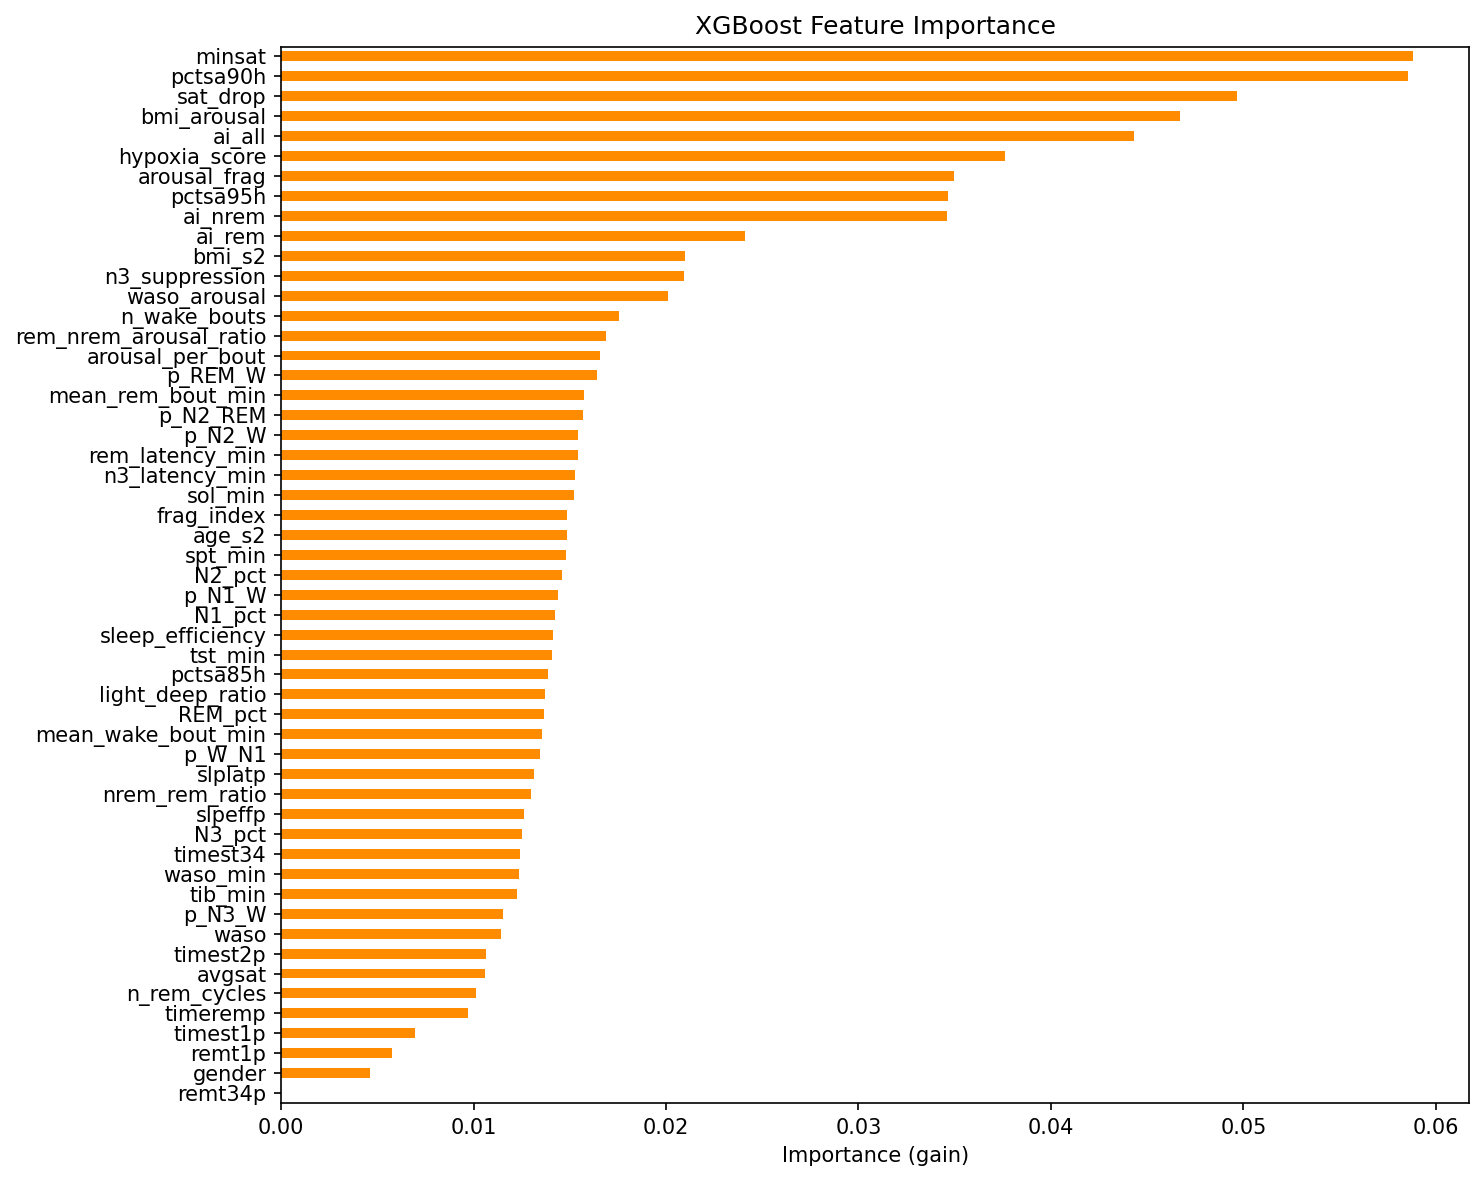
\includegraphics[width=0.86\textwidth]{images/resultats/xgb_feature_importance.png}
\caption[Importance globale des variables]%
        {Importance des variables du modèle de sévérité, mesurée par le gain.}
\label{fig:importance}
\end{figure}

Les variables les plus influentes relèvent de l'oxymétrie et des index d'éveil, ce qui
est physiologiquement cohérent : ce sont les conséquences les plus directes des
événements respiratoires. Les marqueurs d'architecture du sommeil — fragmentation,
proportion de sommeil profond, durée d'éveil intra-sommeil — viennent ensuite et
apportent l'information complémentaire qui justifie la démarche.

Il faut ici rappeler la limite énoncée au chapitre~\ref{chap:etat-art} : ces
attributions expliquent le \emph{modèle}, non le \emph{phénomène}. Une contribution
élevée signale une forte influence sur la prédiction, en aucun cas un lien de
causalité. Le compte rendu remis au praticien porte cette mention.

% =============================================================================
\section{Limites méthodologiques}
% =============================================================================

Trois limites affectent la portée des résultats. Les énoncer relève de la rigueur, non
de la faiblesse : un jury les identifierait de toute façon, et mieux vaut les avoir
analysées.

\subsection{Un découpage au niveau des époques}

Les douze modèles de base ont été évalués sur un découpage \textbf{au niveau des
époques} : les \num{195130} fenêtres ont été réparties aléatoirement entre
entraînement, validation et test, sans tenir compte du sujet dont elles proviennent.
Comme chaque sujet contribue environ un millier d'époques, dont \SI{80}{\percent}
atterrissent dans l'ensemble d'entraînement, le modèle a vu — pour presque chaque
époque de test — d'autres époques du même patient, du même montage et de la même nuit.

Les métriques du tableau~\ref{tab:12modeles} mesurent donc la capacité à classer
\emph{une époque inconnue d'un patient connu}, et non \emph{un patient inconnu}. Elles
surestiment vraisemblablement la performance en situation clinique réelle.

\subsection{Deux protocoles non comparables}

Les ensembles, eux, ont été construits et évalués sur un découpage \textbf{par sujets},
avec \num{20} sujets de test et \num{20} de validation. Il en résulte deux
conséquences.

D'une part, les valeurs du tableau~\ref{tab:ensembles} et celles du
tableau~\ref{tab:12modeles} \textbf{ne sont pas directement comparables} : elles
portent sur des jeux de test différents, de tailles différentes — \num{20314} contre
\num{19513} époques — et de distributions légèrement différentes. Le mémoire ne
présente donc pas le passage de \SI{91,66}{\percent} à \SI{96,93}{\percent} comme un
gain de l'empilement, car ce serait une comparaison invalide.

D'autre part, et c'est plus gênant, les modèles de base ayant été entraînés sur un
découpage par époques, ils avaient déjà rencontré des fenêtres appartenant aux sujets
que le protocole d'empilement considère comme non vus. L'étanchéité recherchée n'est
donc pas parfaite, et les performances des ensembles sont elles aussi
vraisemblablement optimistes.

\subsection{Un corpus restreint et filtré}

Le sous-corpus de 196 sujets représente \SI{3,4}{\percent} de la cohorte disponible,
et il a été constitué par filtrage sur la complétude du montage plutôt que par tirage
aléatoire. La diversité des morphologies, des pathologies et des conditions
d'enregistrement y est donc moindre que dans la cohorte complète.

\subsection{Conséquence et travail correctif prioritaire}

Ces trois limites se renforcent mutuellement et pointent vers un même correctif : une
\textbf{ré-évaluation complète sur un découpage par sujets unique}, appliqué de façon
identique aux modèles de base et aux ensembles, avec un tirage aléatoire des sujets
plutôt qu'un filtrage par ordre. Ce travail, qui ne nécessite aucune modification des
architectures, constitue la première des perspectives.

% =============================================================================
\section{Conclusion}
% =============================================================================

Ce chapitre a présenté la réalisation des deux étages d'apprentissage et leurs
résultats. La stratégie d'entraînement a fait l'objet d'un arbitrage explicite :
restreindre la cohorte pour maintenir le corpus en mémoire vive, et préserver ainsi la
qualité de convergence plutôt que le volume de données.

Sur la classification des stades, le modèle convolutif à cinq dérivations et trois
classes atteint \SI{91,66}{\percent} d'exactitude pour un $\kappa$ de \num{0,853},
au voisinage de l'accord inter-expert rapporté dans la littérature. Le stade N1
constitue le seul échec véritable, avec un F1 de \num{0,26}, ce qui rejoint les
difficultés documentées sur cette classe de transition. L'empilement dépasse le
meilleur modèle isolé sur les quatre configurations, mais ne dépasse le vote moyen que
sur trois d'entre elles.

Sur la prédiction de sévérité, la forêt aléatoire atteint \SI{57,0}{\percent}
d'exactitude pour un $\kappa$ de \num{0,409} sur quatre classes, avec plus de
\SI{95}{\percent} des prédictions dans la bonne classe ou une classe adjacente.
L'empilement n'y apporte aucun gain, résultat négatif que nous avons rattaché au
défaut de diversité entre des modèles tous fondés sur des arbres.

Enfin, trois limites méthodologiques ont été analysées, dont la principale — un
découpage au niveau des époques et non des sujets — conduit vraisemblablement à
surestimer la performance en situation clinique. La ré-évaluation correspondante
constitue la première perspective de ce travail.

Le chapitre suivant décrit la plateforme qui met ces modèles à disposition des
praticiens, et son déploiement.
